\section{Background}
\label{sec:background}

% <intro>

\subsection{Large Language Models}
% Intro
A Large Language Model (LLM) is a model of Artificial Intelligence (AI), based on neural networks, designed to understand and generate text in natural language.

These models are based on the transformer architecture \cite{vaswani2023attentionneed}, which uses a self-attention mechanism to capture relation of words in a sequence.
They are implemented as autoregressive models, and are characterized by a large number of parameters, often reaching billions, which, combined with training on massive amounts of textual data, enables them to perform a variety of complex linguistic tasks.
Their behavior relies on next-token prediction: given a textual context, they predict the next one in sequence, token after token, until the desired output is complete.

% History and common models
\medskip
With GPT-2 \cite{radford2019language}, OpenAI showed that a model trained on large quantities of texts can generate very coherent output.
GPT-3 \cite{brown2020LMfewshot}, with 175 billions of parameters, highlighted emergent behaviors such as few-shot learning, which is the ability to perform new tasks by simply observing few examples in the prompt.
Since then, many LLMs have been presented, including LLaMA and Claude, each one with similar architectures but different optimizations \cite{wang2025llm}.

While the scientific emergence has been driven by the scale of the model, the wide diffusion has been possible by the ease of use through accessible conversational interfaces, such as ChatGPT, which enabled these models to be used also by non experts, thanks to the use of prompts in natural language and the accessible interface.

% Tasks and applications
\medskip
One of the main reasons why LLMs are so popular is their ability to adapt to a wide variety of applications.

A general LLM, trained on large quantities of data, can be further specialized through a phase of fine-tuning on specific data, to adapt it to a specialized domain by simply providing new data about the topic of interest.

An example is BloombergGPT \cite{wu2023bloomberggptlargelanguagemodel}, an LLM developed and optimized on a large corpus of proprietary financial data. This model showed better performances with respect to generalized LLMs in financial tasks, such as the analysis of economic documents or the generation of reports, confirming that fine-tuning helps improving the coherence of the generated content in specific contexts \cite{wang2025llm}.

\medskip
Other common applications include the automatization of linguistic tasks, such as translation, summarization and content generation. LLMs are used for conversational systems like customer assistance, and as personal assistants.
Other applications include:
\begin{itemize}
    \item scientific research: they help analyzing literature, synthesizing articles and identifying relevant information in a large corpus of texts;
    \item education: they support students and teachers by generating clearer explanations and didactic material;
    \item medicine: they can support decision, and suggest possible diagnosis, based on the given data \cite{wang2025llm}.
\end{itemize}

\medskip
Even though these models were initially designed to work only on texts, they are rapidly evolving toward a new multimodal format, enabling them to elaborate and generate content including images, audios and videos, integrating a wide diversity of information.


% Limitations
\medskip
Even though LLMs offer numerous advantages, it's important to also consider the limitations that this technology presents.

One of the main problems is the high computational cost required to train large models.
This process demands extensive hardware resources and significant energy consumption, with raises environmental concerns.

Another major limitation concerns the quality of the generated contents. Although the outputs are often grammatically correct and believable, they are not always accurate or reliable. Models can produce inaccurate or false information, a phenomenon known as \textit{hallucinations}, which can be problematic in domains where precision is critical, such as medicine.

A related concern is security: LLMs may generate content that is harmful, inappropriate or offensive. This raises ethical issues and requires appropriate control to guarantee responsible use of these models.

Another challenge lies in the need to formulate effective prompts. While these models can understand natural language, the syntax and the semantic of the prompts can affect the output. This phenomenon requires a careful prompt engineering, in order to get higher-quality responses.

Moreover, the lack of explainability is a significant limitation. LLMs are complex systems, and their black-box nature makes it difficult to understand and justify the reasoning behind their outputs.

Finally, privacy is another frequently discussed issue. During the training phase, LLMs may be exposed to sensitive data, which could potentially be reproduced in later outputs. This raises concerns about data misuse and highlights the need for clear rules to protect personal information.


\subsubsection{LLMs in Agent-Based Modeling}
% What it is
Agent-Based Modeling (ABM) is a method used to simulate complex systems starting from the behavior of single individuals, called agents.
Each agent acts according to specific rules, and the interaction between multiple agents enables the emergence of collective phenomena and global dynamics.
This mechanism makes it possible to study how local behavior, at individual level, can have an impact on the raise of phenomena on a large scale, passing from a micro to a macro level.

ABMs are widely used in the study of social phenomena, such as information diffusion, group dynamics, or the emergence of complex social structure.

% Limitations of traditional ABMs
\medskip
However, traditional ABMs have some limitations.
Agents are generally described by a set of simple and fixed rules, which prevents them from adapting to new situations or reason autonomously \cite{conte2014agent, törnberg2023evaluate}.
This makes it hard to realistically represent human behavior. Specifically, agents lack some important aspects of communication and social interactions, such as the tone, the emotions, or the ability to develop a personal idea based on the context.
These limitation are mostly evident when trying to simulate complex social contexts, like digital platforms, where the the interactions are influenced by the language and multiple other external factors.

% LLM potential
\medskip
In the last years, however, LLMs have started to be integrated in Agent-Based systems.
These models allow to define more complex and realistic agents: they can generate text, discuss, express opinions and reason on a given topic. 
In this way, agents are more similar to real individuals.
Moreover, LLMs can be designed to impersonate specific given profiles. They can have their own personality, emotions, political leaning and memory of the interactions, and behave accordingly.

For these reasons, LLMs provide the means to realistically simulate complex phenomena at both individual level (for example with confirmation bias), and at global level (for instance with polarization and echo chambers).

\medskip
This recent integration of LLMs and ABM was at the basis of many advanced social simulators.
Among these, there is also Y simulator, presented by \citet{rossetti2024ysocialllmpoweredsocial}, at the basis of this work.
In Y, each agent is represented by an LLM, who can perform the complex actions typical of a social media (including posting, replying and following other users), and interact with other agents, coherently with the assigned profile.
User profiles are also enriched with personal information such as interests, political leaning, demographic data and personality, which contribute to make the simulation realistic.


% AutoGen
\subsubsection{AutoGen: multi-agent conversation framework}
AutoGen is an open-source library developed by Microsoft, presented by \citet{wu2023autogenenablingnextgenllm}, to facilitate the creation of environments where LLM-based agents can interact.
This framework has been designed to support the creation of multi-agent conversations, with coherent and realistic multi-turn conversations. 

\medskip
The system is easily accessible thanks to the Python interface \cite{pyautogen0.2.31}, which allows developers to design complex communication flows.
For these reasons, AutoGen is very effective for simulating users in simulated social environments like social networks, where interactions play a central role.

\medskip
This work simulates a social platform using Y\cite{rossetti2024ysocialllmpoweredsocial}, which is based on AutoGen to design and orchestrate agents.
Specifically, it uses \textit{AssistantAgent}, a type of agent designed to answer and interact based on specific prompts.
Each user is an LLM-based agent, initialized with a personalized with a profile, including opinions and communication style.
Using AutoGen allows orchestrating conversations among agents in a natural way, enabling the emergence of realistic dynamics.


% Personality
\subsubsection{Personality modeling}
One of the main advantages of using LLMs to simulate social behavior is the possibility to enrich each agent with profile details.
This allows differentiating the behavior of individuals in a simulated population, contributing to make the environment more realistic.

Among the characteristics that can be integrated in the agent initialization phase, one of the most significant is personality.
Including personality traits makes it possible to model agents that act coherently with their own identity.
This is especially significant in social simulations, since human behavior is influenced not only by the content received, but also in the way they interact, answer and make decisions.

\medskip
The most well-known and used personality model is the Big Five Model, or the Five Factors Model \cite{barrick1991bigfive, McCrae1992}. This approach describes human personality in five main dimensions, which are present in each individual in different levels:

\begin{itemize}
    \item \textbf{Openness to Experience}: it measures the tendency to being curious, creative and open to new ideas and experiences. People with a high score tend to appreciate art and imagination, while who has a low score can be more practical and routine-oriented.
    
    \item \textbf{Conscientiousness}: it indicates the degree of organization, precision and self-discipline. Conscientious individuals are reliable, they plan everything carefully and follow rules, whereas those with a low score can be more impulsive and unorganized.
    
    \item \textbf{Extraversion}: it concerns the tendency to be sociable and assertive. Extroverts enjoy social interactions, whereas introverts prefer quiet and solitary environments. 
    
    \item \textbf{Agreeableness}: it measures the tendency of being kind, empathic and cooperative. People high in agreeableness tend to be cooperative, while those with a low score can be competitive and critical.
    
    \item \textbf{Neuroticism}: it reflects the predisposition to fell negative emotions like anxiety, anger or depression. Individuals high in neuroticism can feel stress and external pressure, while those with a low score tent to be more emotionally stable. 
\end{itemize}


\medskip
Integrating these traits in the design of LLM agents helps simulating not only the different static behaviors, but also the different levels of susceptibility to social influence.
In social network contexts, people don't behave in the same way when facing to controversial content or different group dynamics.
Personality plays a crucial role in determining how much an individual is susceptible.

\medskip
\citet{oyibo2019personality} studied the relation between personality traits and the susceptibility to social influence, showing that Neuroticism, Openness and Conscientiousness are the most relevant factors.
The study highlights that individuals with high Neuroticism tend to look for external approve, and are therefore more inclined to conform to others' opinions to avoid conflicts.
People with high Openness are more open to accept new or different points of view, resulting in a higher susceptibility to influence.
On the contrary, individuals high in Conscientiousness tend to think before changing their views, and are less impulsive in modifying their ideas.

\medskip
These insights underscore the value of integrating personality dimensions in agent modeling, with Big Five traits providing a robust mean to capture behavioral diversity in simulations.




\subsection{Opinion dynamics}
% Intro
One of the crucial aspects when studying social behavior is understanding how people evolve their opinions over time, especially when interacting with others.
Opinion dynamics aims at describing these mechanisms, using theoretical and computational models.
The goal is to explain how opinions spread in a population, how people influence each other, and under which conditions phenomena like consensus and polarization emerge.

Additionally, it has become even more relevant in the age of social media, where the interactions among individuals are large-scale and fast.
Understanding opinion dynamics helps explaining complex phenomena like disinformation diffusion and echo cambers, and it's is useful in many areas, like sociology, psychology, network science and artificial intelligence.


% Tradutional models
\medskip
The first approaches proposed to describe opinion dynamics focus on capturing how individuals are influenced by the opinions of others within their social environment.

One of the most well-known traditional models is the one presented by \citet{Degroot1974}, according to which the opinion of an individual is the weighted average of the opinions of its neighbors in the network:

\[
x_i(t+1) = \sum_{j=1}^n w_{ij} \, x_j(t)
\]

where $x_i(t)$ is the opinion of $i$ at time $t$, $w_{ij}$ is the weight of individual $j$ on $i$, with $\sum_{j} w_{ij}=1$.

This model has been widely used as a theoretical foundation of studies on information spread and social network analyses. However, it presents a limitation: it doesn’t consider the tendency of an individual to keep the initial opinion.

For this reason, the model by \citet{friedkin_1990} introduces the concept of \textit{stubbornness}, modeled with a susceptibility parameter $\lambda$:

\[
x_i(t+1) = (1 - \lambda_i) \, x_i(0) + \lambda_i \sum_{j=1}^n w_{ij} \, x_j(t)
\]

where $x_i(0)$ is the initial opinion and $\lambda_i \in [0, 1]$ is the susceptibility of $i$ to influence.
Therefore, this model allows to consider individuals with different levels of stubbornness, describing how inclined they are to change their idea.

Other variants exists, such as state-dependent models, where the opinion update is anchored to the individual's current opinion, instead of the initial one.


% Limitations
\medskip
Even though these traditional mathematical models are simple and effective, they present some limitations in accurately representing the complexity of social behavior.
First, they reduce the opinion to a single numerical value, and its evolution to a deterministic formula, leaving out many aspects typical of human interactions.
They don't take into consideration, the context and the individual's personality and language.
Moreover, they tend to oversimplify the network, and don't give importance to emotional tone and the modality of the interaction (in a social network, for instance: \textit{like}, \textit{comments}, \textit{follow}).

For example, in a real-world political discussion an individual acts according not only on the stance of the other person, but also on the tone in which the opinion is expressed (kind, ironic, aggressive), or external factors, such as the authority of the source.
Traditional mathematical models lack all these aspects.


% Modern solutions (LLMs)
\medskip
To overcome these limitations, in the last years LLMs have been widely adopted as agents in social simulations.
LLMs can read, write, and reason on a given context, just like normal users would do.
They can be programmed to answer in a way which is coherent with an assigned profile, for example representing an individual with a specific personality or political opinions.
This enables more realistic simulations, where the opinion is not a simple abstract number, but is expressed in natural language, and can be influenced by the tone, the content and the context of the received information.

\medskip
As shown by \citet{chuang2024simulatingopiniondynamicsnetworks, cau2025languagedrivenopiniondynamicsagentbased, piao2025emergencehumanlikepolarizationlarge}, this approach allows to observe phenomena which would be hardly reproducible with traditional mathematical models, such as confirmation bias, polarization, and consensus.
Furthermore, LLMs can integrate other aspects, including a memory of the interactions, the agents' personality (modeled, for instance, with the Big Five), or the tendency to believe in fake contents.
In this way, the agents' behavior becomes more similar to the humans' one, and the simulations' results are better and easier to interpret even for an external human observer.

\medskip
The next sections will dive deeper into both the computational models used to represent opinions, and how LLMs are used to simulate believes and realistic behaviors in a complex social context.





\subsection{Misinformation and disinformation} % 1
Recently, the spread of misleading content has become meaningful, mainly due to the massive diffusion and use of social media.
To speak about this topic correctly, it is important to clarify the definitions of \textit{misinformation}, \textit{disinformation} and \textit{malinformation}, since they are often used together, even though they are distinct phenomena.


According to the definition proposed by \citet{wardle2017information, wardle2017information}, \textit{disinformation} is false information that is deliberately created or disseminated with the express purpose to cause harm.
For instance, the creation of an event that didn't occur, to manipulate public opinion.

\textit{Misinformation} is instead when false information is shared, but no harm is meant: for example, someone shares a news, without knowing it's false.

A third type, less known but equally present, is \textit{malinformation}: in this case the information is true, but it's shared with the purpose to cause harm, for example when information designed to stay private is shared publicly.

The main difference stands therefore both in the information truthfulness and in the intention of who shares it. This classification is shown in Fig \ref{fig:info_disorder}, and is taken from \cite{wardle2017information}.

\begin{figure}[h]
    \centering
    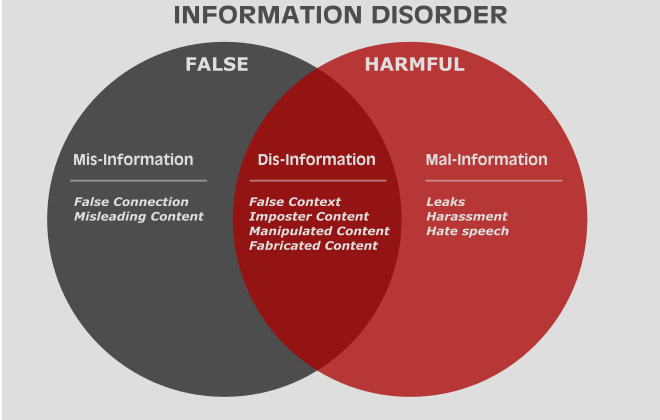
\includegraphics[width=0.5\linewidth]{Images/information_disorder_Wardle.png}
    \caption{Figure from \cite{wardle2017information}, showing the difference among different types of information disorders.\\
    \textit{Misinformation}: false information is shared, but no harm is meant. \textit{Disinformation}: false information is knowingly shared to cause harm. \textit{Malinformation}: genuine information is shared to cause harm.}
    \label{fig:info_disorder}
\end{figure}


Although misleading content has always existed, the rise of social media platforms has significantly amplified both their diffusion and impact. 
Events such as the 2016 USA presidential elections and the Brexit referendum are considered among the earliest large-scale representative cases of disinformation campaigns.

Over the past decade, the spread of false or misleading information has intensified, due to multiple key factors.
Social media enable anyone to create and share content, often without any form of confirmation. The rapid diffusion is further simplified by the speed and easy at which information can circulate.
Moreover, fake content is typically easier to produce, but harder to detect \cite{aimeur2023fake}. 

\medskip
A research by \citet{kumar2018falseinformationwebsocial} highlights that tweets containing false information tend to reach more users and spread more quickly compared to truthful content. The study also emphasizes that political topics are among the most frequently targeted by disinformation.

In many cases, the diffusion of false content is amplified due to a significant delay between the publication and its debunking: it generally takes around 12 hours to correct a false information, and during this time it can spread and even become viral, and this is particularly true for content that seems trustworthy and sometimes is occasionally shared by trusted sources.

\medskip
Platforms like Facebook and Twitter allow the diffusion of false information, due to the absence of editorial filters and the ease with which anyone can participate in spreading content \cite{hilary2021social}.
The contributors to the diffusion can be either unintentional users or even organizations with political, economic, or ideological purpose.

The consequences of these mechanisms are not limited to individuals alone: they can increase polarization, reduce trust, and have a negative impact on political debates.









\subsection{Italian political context (2022)} % 1
% Including coalitions and topics used in this study
